\documentclass{beamer}
\usepackage[latin1]{inputenc}
\usepackage{tikz}
\usepackage{qtree}
\usetheme{Warsaw}
\title[Lisp Interpreter]{Full Lisp Interpreter}
\author{Shun Zhang\\ Wang Rao\\ Zeyuan Zhu}
\begin{document}

\begin{frame}
\titlepage
\end{frame}

\begin{frame}{Features}
\begin{itemize}
\item AST built by hand, without \texttt{jjtree}.
\item Curried functions (i.e. every lambda expression on the AST has only one argument).
\item Each node has its own environment.
\item Multiple, extensible visitors (easy to add a \texttt{SQLInsertionVisitor}, if needed).
\item Static/Dynamic scoping.
\end{itemize}
\end{frame}

\begin{frame}{Structure}
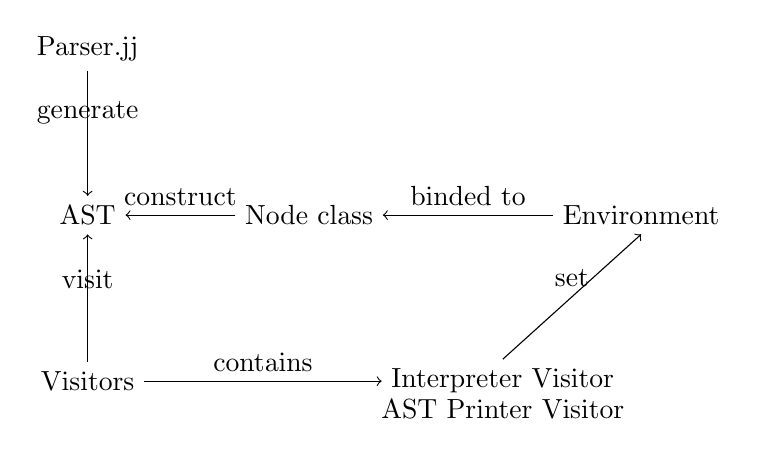
\begin{tikzpicture}
  [ ->, above, node distance=6em]
  \node [name=parser] {Parser.jj};
  \node [name=ast, below of=parser] {AST};
  \node [name=visitor, below of=ast] {Visitors};
	\node [name=node, right of=ast, node distance=8em] {Node class};
	\node [name=env, right of=node, node distance=12em] {Environment};
	\node [name=visitors, right of=visitor, node distance=15em] { Interpreter Visitor};
	\node [name=visitors2, below of=visitors, node distance=1em] {AST Printer Visitor};

  \path (parser.south) edge node {generate} (ast)
				(visitor.north) edge node {visit} (ast)
				(node.west) edge node {construct} (ast.east)
				(env.west) edge node {binded to} (node)
				(visitor.east) edge node {contains} (visitors.west)
				(visitors.north) edge node {set} (env.south);
\end{tikzpicture}
\end{frame}

\begin{frame}{Visitor}
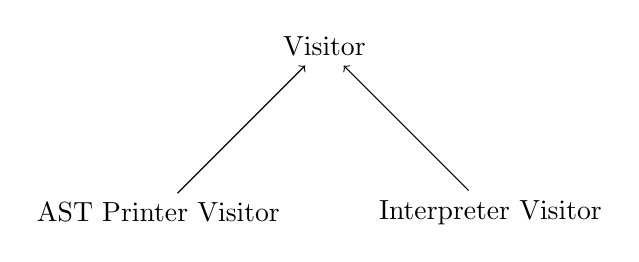
\begin{tikzpicture}
  [ ->, above, node distance=6em]
	\node [name=super] {Visitor};
	\node [name=ast, below of=super, left of=super] {AST Printer Visitor};
	\node [name=interp, below of=super, right of=super] {Interpreter Visitor};

	\path (ast) edge (super)
				(interp) edge (super);
\end{tikzpicture}
\hfill \\
\begin{itemize}
\item Interpreter Visitor: Evaluate each node, print out its environment, and the final result.
\item AST Printer Visitor: Print out what it sees on the AST.
\end{itemize}
\end{frame}

\begin{frame}{Grammar}
$Lambda \rightarrow (lambda\ ((Id)*)\ Expression|Lambda) $\\
\hfill \\
$Application \rightarrow (Lambda|Application\ \{Expression|Lambda\})$\\
$|\ (let\ ((Id\ Expression|Lambda)*)\ Expression|Lambda)$\\
\hfill \\
$Addition \rightarrow (+\ (Expression)*)$\\
\hfill \\
$Expression \rightarrow Application | Addition | Id | Number$\\
\end{frame}

\begin{frame}{AST: Lambda}
$(lambda\ (id)\ expression)$
\hfill \\
\hfill \\
\hfill \\
\Tree [.$\lambda$ [.id ] [.expression ] ]
\end{frame}

\begin{frame}{AST: Application}
$(lambda\ expression)$ \\
\hfill \\
\hfill \\
\hfill \\
\Tree [.app [.lambda ] [.expression ] ]
\end{frame}

\begin{frame}{AST: Application}
$(let\ ((id\ expression))\ body)$ \\
\hfill \\
\hfill \\
\hfill \\
\Tree [.app [.$\lambda$ [.id ] [.body ] ] [.expression ] ]
\end{frame}

\begin{frame}{AST: Addition}
$(+\ expression1\ expression2\ ..\ expressionN)$ \\
\hfill \\
\hfill \\
\hfill \\
\Tree [.+ [.expression1 ] [.expression2 ] [. ... ] [.expressionN ] ]
\end{frame}

\begin{frame}{Example}
(let ((x 3)) (let ((f (lambda (y) (+ x y)))) (f 4)))\\
\hfill \\
Or ((lambda (x) ((lambda (f) (f 4)) (lambda (y) (+ x y)))) 3)\\
\hfill \\
\Tree [.app [.$\lambda$ [.x ] [.app [.$\lambda$ [.f ] [.app [.f ] [.4 ] ] ] [.$\lambda$ [.y ] [.+ [.x ] [.y ] ] ] ] ] [.3 ] ] \\
\hfill \\
Demo: Input\_sample
\end{frame}

\begin{frame}{Environment}
\begin{itemize}
\item Each node has its own environment.
\item Envrionment is passed down along the AST when interpreter is visiting.
\item When interpreter sees an Application, it constructs an ASub object and appends it to the environment.
\item ASub has two types: simple ASub and closure ASub.
\end{itemize}
\end{frame}

\begin{frame}{Preloaded Functions: car, cdr, cons}
Functions of \texttt{car, cdr, cons} can be preloaded in to environment by \texttt{-p} flag. They will appear at the envrionment of the root of AST.\\
\hfill \\
Example: function cons appears as\\
\hfill \\
\Tree [.$\lambda$ [.elem ] [.$\lambda$ [.list ] [.body ] ] ]  \\
\hfill \\
Demo: Input\_list
\end{frame}

\begin{frame}{Preloaded Functions: Combinators}
All combinators are also preloaded. Their definitions are stored in a \texttt{Preload} file in the following format.
\texttt{Parser.jj} will parse \texttt{Preload} file first to load these functions into environment.
\hfill \\
\hfill \\
Parse them by 
\texttt{(<ID> <ASSIGN> lambda())*}
\hfill \\
\hfill \\
\texttt{s := (lambda (f g x) (f x (g x)))}\\
\texttt{k := (lambda (x y) x)}\\
\texttt{b := (lambda (f g x) (f (g x)))}\\
\texttt{c := (lambda (f g x) (f x g))}\\
\texttt{y := (lambda (f x) (f (y f) x))}\\
...\\
\texttt{pradd1 := (lambda (x z) (y (b (condzero (k z)) (b (s (b plus (k 1))) (c b pred))) x))}\\
...\\
\end{frame}

\begin{frame}{Preloaded Functions: Combinators}
For example: \texttt{s f g x = f x (g x)}. The structure it appears in the environment is\\
\hfill \\
\hfill \\
\Tree [.$\lambda $ [.f ] [.$\lambda $ [.g ] [.$\lambda $ [.x ] [.app [.app [.f ] [.x ] ] [.app [.g ] [.x ] ] ] ] ] ]
\end{frame}

\begin{frame}{Multiple Binding of Let, Lambda}
\begin{itemize}
\item Translate multiple binding of lambda to curried function in the parser.
\item Application can return function.
\item Clean AST structure.
\end{itemize}
\end{frame}

\begin{frame}{Multiple Binding of Let, Lambda : Example}
(let ((x 1) (y 2)) (+ x y)\\
Or ((lambda (x y) (+ x y)) 1 2)\\
$\rightarrow$ (((lambda (x) (lambda (y) (+ x y))) 1) 2)
\hfill \\
\hfill \\

\Tree [.app [.app [.$\lambda$ [.x ] [.$\lambda$ [.y ] [.+ [.x ] [.y ] ] ] ] 1 ] 2 ]
\hfill \\
Demo: Input\_multi\_lambda Input\_multi\_let
\end{frame}

\begin{frame}{Multiple Binding of Let, Lambda : Implementation}
\begin{verbatim}

<LPAR> <LAMBDA> <LPAR> (t = <ID> \{ tlist.add(t.image); \})* <RPAR>  

(LOOKAHEAD(2)  exp = expression() | exp = lambda() ) <RPAR>

\{ 

	for ( int i = tlist.size() - 1; i >=0; i-- )

	\{

			exp = new Lambda(tlist.get(i), exp);

	\}

	return (Lambda)exp;

\}
\end{verbatim}
\end{frame}

\begin{frame}{Static/Dynamic Scoping}
For example, f is found in the envrionment as \texttt{(lambda (x) (+ x 1))} and interpreter sees \texttt{(f 3)}\\
\Tree [.app [.f [.$\lambda$ [.x ] [.+ [.x ] [.1 ] ] ] !{\qframesubtree} ] [.3 ] ]
\hfill \\
\hfill \\
\begin{itemize}
\item Static scoping : as it is.
\item Dynamic scoping : + node using the environment of $app$ node.
\end{itemize}
\hfill \\
Demo: Input\_scope
\end{frame}

\begin{frame}{Recursion}
Example \\ \texttt{(letrec ((f (lambda (n) (if0 n 1 (+ (f (+ n -1)) n))))) (f 2))} \\
\Tree [.app [.$\lambda$ [.f ] [.app [.f ] [.2 ] ] ] [.$\lambda$ [.n ] [.if0 [.cond ] [.then ] [.else ] ] ] ] 
\end{frame}

\begin{frame}{Recursion}
\begin{itemize}
\item If defined by \texttt{letrec}, put a copy of the function definition into its environment.
\item Example \\ \texttt{(letrec ((f (lambda (n) (if0 n 1 (+ (f (+ n -1)) n))))) (f 2))} \\
\hfill \\
Intuition: $f=
\begin{cases}
1,\ if\ n = 0 \\
f(n-1)+n,\ otherwise
\end{cases}$
\hfill \\
\hfill \\
$f(2)=2+f(1)=2+1+f(0)=2+1+1=4$
\end{itemize}
\hfill \\
Demo: Input\_rec
\end{frame}

\begin{frame}{What we learnt}
\begin{itemize}
\item Visitor design pattern.
\item Mechanism of interpreter.
\item Deep understanding of object-oriented programming.
\end{itemize}
\end{frame}
\end{document}
